\documentclass[a4paper, 11pt]{report}
%\usepackage{fontspec} % needs to be in main.tex
\usepackage{lmodern}


\usepackage[top=2.5cm, bottom=2.5cm, left = 2cm, right = 2cm]{geometry} 
\geometry{a4paper} 
\usepackage[utf8]{inputenc}
\usepackage{textcomp}
\usepackage{graphicx} 
\usepackage{amsmath,amssymb, amsfonts, amsthm}  
\usepackage{bm}  
\usepackage[pdftex,bookmarks,colorlinks,breaklinks]{hyperref}  
\usepackage{memhfixc} 
\usepackage{pdfsync} 
\usepackage{fancyhdr}
\pagestyle{fancy}
\usepackage[backend=biber,style=numeric,sorting=none,minbibnames=1]{biblatex}
\renewcommand{\familydefault}{\sfdefault}
\usepackage{float}
\usepackage[section]{placeins}
\usepackage{xurl}
\usepackage{xcolor}
\usepackage{colortbl}
\usepackage[export]{adjustbox}
\usepackage{subcaption}
\usepackage{hyperref}

\addbibresource{references.bib}
\graphicspath{{figures/}}

% Command for new paragraph
\newcommand{\p}{\par\bigskip\noindent}

% No indent at start of paragraph
\setlength\parindent{0pt}

% URL style
\hypersetup{
    colorlinks=true,
    linkcolor=blue,
    filecolor=magenta,
    urlcolor=cyan,
}
\urlstyle{same}

% Title page with image
\title{
    {\Huge Ergonomic Posture Detection}\\
    {\large Business Values - Prof. Dr. Sandra Dressler}
}
\author{Nourhan Omar, Vipin Singh, Polina Kozyr, Pavlo Kravets, Ari (Sara) Wahl}
\date{
    \begin{figure}[h]
        %\centering
        
\includegraphics[width=17.5cm,height=17.5cm]{test}
    \end{figure}
}


\begin{document}
    \begin{titlepage}
    \begin{center}
        \vspace*{1cm}
        
        \Huge
        \textbf{Ergonomic Posture Detection}
        
        \vspace{0.5cm}
        \LARGE
        \textbf{Business model documentation}
        
        \vspace{1.5cm}
        \Large
        \textbf{Group:}\\
        Ari (Sara) Wahl, Nourhan Omar, Pavlo Kravets, Polina Kozyr, Vipin Singh
        
        \vfill
        
\includegraphics[width=\textwidth]{cover_image.png}
        \vfill
        
        \Large
        Business Values - Prof. Dr. Sandra Dressler\\
        Master Data Science - Winter Term 23/24\\
        Berliner Hochschule für Technik
        
    \end{center}
\end{titlepage}

    % Abstract
	{
		\FloatBarrier
		\newpage
        \setcounter{page}{2}
		\phantomsection
		\addcontentsline{toc}{chapter}{Abstract}
		\thispagestyle{plain}
		\vspace*{\fill}
			\section*{{\Large Abstract}}
			Test\cite{dummy}
		\vspace*{\fill}
	}

    % Table of contents
    {
        \FloatBarrier
        \newpage
        \phantomsection
        \addcontentsline{toc}{chapter}{Contents}
        \tableofcontents
    }

    % Introduction: What is the problem?
	{
		\FloatBarrier
		\chapter{Introduction}
		\label{chp:introduction}
		\documentclass{article}

\begin{document}

\section*{Introduction}

(by Nourhan Omar)\\

In today's digital age, the widespread use of computers has become an integral part of daily life for many people, whether for work, studying, or playing video games. However, given the convenience and mobility offered by laptops, the importance of maintaining good posture often gets overlooked, resulting in a lot of health issues such as back pain and frequent visits to physiotherapists.

Despite efforts by some companies to address this issue by providing ergonomic furniture and standing desks, employees still face challenges in maintaining optimal posture throughout their workday. The shift to remote or hybrid work arrangements following the COVID-19 pandemic has only increased this problem, as many individuals now rely on home office setups that probably lack ergonomic design.

Moreover, the high cost of ergonomic furniture can pose a barrier for both employers and individuals, making it impractical. While exercises and stretches can help with posture-related pain, the demands of a busy workday often leave little time for dedicated physical activity.

Considering these challenges, there is a pressing need for innovative solutions that can easily integrate into work environments, promoting healthy posture habits without affecting overall productivity. By addressing the root causes of poor posture and providing practical, accessible solutions, we can empower individuals to prioritize their physical health and overall well-being.

\end{document}

	}

    % Solution: How to address this need?
	{
		\FloatBarrier
		\chapter{Solution: How to adress this need?}
		\label{chp:solution}
		(by Ari Wahl)

The first goal of this project is to develop a software that helps people to work
ergonomically correct. We will develop an application that will be able to detect the user's posture in real-time
and give feedback to the user. The feedback should be given in a way that users
can correct their posture if necessary. The software should be easy to use and should be able to run on 
different platforms and devices. It should be available and easily accessible to businesses and private users. Ideally, the user
can just use the webcam of their device to use the software. The application will be able to run in the background
and give the feedback in a subtle way. We propose a traffic light colored-scheme that will be displayed as a frame
around the users screen. This means that the frame will be green if the user's posture is correct, yellow if the posture is not optimal 
and should be changed soon and red if the posture is bad and should be changed immediately. 
We will also provide an option to display the feedback as sound. There will be no sound if the posture is correct, a
beep from time to time if the posture is not optimal and a continuous sound if the posture is bad.

As data privacy is an important issue with real-time video analysis, we will develop the software in a way that the raw video data
will not leave the user's device. It will be processed locally in a first step on the user's device and only the processed data will be sent to the server.

To further develop our application we will (optionally) also analyse the data over time and give the user feedback about their posture 
in the form of a dashboard. This dashboard will show the user for example how much time they spent in a good, bad or neutral posture
and which is their most used bad posture, etc. It will also show the user how much time they spent sitting in total. 

As a further step, the application will be extended to optionally also give the user advice on how to compensate for long sitting periods.
This will be done by suggesting the user different exercises once in a while after they have been sitting for a long time.  

For further development we see the potential to grow into an ergonomic workout application branch. This means that
we will have an additional model to detect the user's posture and movements during workout and give them feedback on how to do the exercises correctly.

Another possible area of growth will be physiotherapy applications. 
This means that we will have an additional model to detect the user's posture and movements
during physiotherapy exercises and give them feedback on how to do the exercises correctly.

Since these further developments need additional resources and domain knowledge we will focus on the implementation
of the first goal of this project. 
	}

    % Technology: Why is it unique?
	{
		\FloatBarrier
		\chapter{Technology: Why is it unique?}
		\label{chp:technology}
		
Notes by Ari

- main model:
state-of-the-art model for pose estimation from papers with code
or alternatively:
YOLO runs live within the app on the device of the user, outputs the keypoints and we only classify on those, meaning only the keypoints are sent to the cloud, which is probably a decent abstraction...

- fine tuning:
with own dataset according to RULA

- data privacy:
We need to ensure that the privacy of our customers is kept safe. Therefore we propose a preprocessing of the videofeed within the app to so that only privacy-preserved data leaves the users device and ends up in the cloud where it is inserted into the machine learning model.

Privacy-Preserving Machine Learning with Fully Homomorphic Encryption for Deep Neural Network:
https://arxiv.org/pdf/2106.07229.pdf
python implementation for homomorphic encryption: [PySeal](https://github.com/Lab41/PySEAL)

or:

* https://easyeasy.medium.com/protecting-privacy-a-comprehensive-guide-to-video-anonymization-for-ai-training-4b85fb23a61d

maybe use a GAN and do a style transfer on the user end: (probably easier to just use the pose estimation on the mobile phone and send only calculated keypoints - of closest human to the camera?)

* https://openaccess.thecvf.com/content/CVPR2023W/ECV/papers/Jia_BlazeStyleGAN_A_Real-Time_On-Device_StyleGAN_CVPRW_2023_paper.pdf

or federated learning approach:
https://github.com/OpenMined/PySyft

- which XAI Method to detect which bodypart is wrongly positioned?
- Advice with arrows in the image on how to correct the posture?

- dashboard with which packages?

- eventually get TÜV certification?

	}

    % Business Model: How to capture value?
	{
		\FloatBarrier
		\chapter{Business Model: How to capture value?}
		\label{chp:business_model}
		(by Pavlo Kravets)

\p
Different segments of the market require different strategies to capture value effectively. Our possible B2B customers would have different motivations, requirements and resourses than our B2C customers. As such, we need to rely on different business models.

\section{B2C}

For the B2C market we are employing a Freemium business model. We are separating our B2C customers into 2 groups: the subscribers and the free users.

\p
Free users will be periodically shown interstitial ads, while the subscribers will have ad-free experience. Interstitial ads vary in price quite a lot: the price depends on customers location, platform, current market demand, etc. According to the report provided by Marc Llobet Rodriguez\cite{ECPM}, in Q3 of the 2023 the CPM (cost per mille) for interstitial ads in developed countries was between 10 and 16 euros. In our calculations we assume this holds true in the future and use a CPM of 13€.

\p
Subscribers, on the other hand, will not be shown any ads. They will be paying a yearly subscription price instead. The price may be adjusted with various promotions, but we assume that the average yearly subscription price will be 15€. Besides the ads removal, users maz be enticed to subscribe by offering various add-ons and premium features.

\p
One of the key problems in B2C market is customer churn. The 30-day retention rate for healthcare apps was 3.7\% according to research\cite{churn}. As such, yearly subscription has several advantages over the monthly one:
\begin{itemize}
    \item It helps to capture more value from the impulsive purchasers. A healthcare app spending may be driven by an acute problem - for example, a period of intense neck pain. Such customers may cancel monthly subscription after the end of the acute episode
    \item It may lead to a stronger habit. The user may utilize the app more if they have already invested into yearly subscription - which, in turn, makes them more used to the app
    \item Some customers may find a single yearly payment less worrying than a monthly expense. They will have a constant reminder of a positive sides of the app, not of the price they pay for it
\end{itemize}

High rates of customer churn and relatively unknown market leads us to believe that we will see exponential growth in active users during the initial period, which turns to linear as time progresses.

\section{B2B}
For the B2B market, we will be mostly employing subscription and one-time payment models, depending if the business customer would prefer to have support or not.

\p
Other possible revenue stream is selling add-ons and customization packages. A lot of businesses may have unique or semi-unique technical requirements. Those requirements can be priced on case-by-case basis, developed and delivered to the customer.

\p
Most businesses prefer to work with well-established countragents. This, as well as possible huge swings in the earnings depending on customer's size and requirements make estimations extremely imprecise. As such, B2B segment is not taken into concideration for calculating the business plan.

\section{Legal structure}
The legal structure chosen for the company is GmbH. It provides limited liability.

\p
As discussed in chapter \ref{chp:team_structure}, there are 5 founders in the company. It makes no financial sense for those founders to pay themselves salaries out of their own pocket, so they will forego salaries. This makes the expenses much lower, but means that the alternative should be calculated: how much would those people earn working as an employee in another company?

\begin{figure}[H]
    \centering
    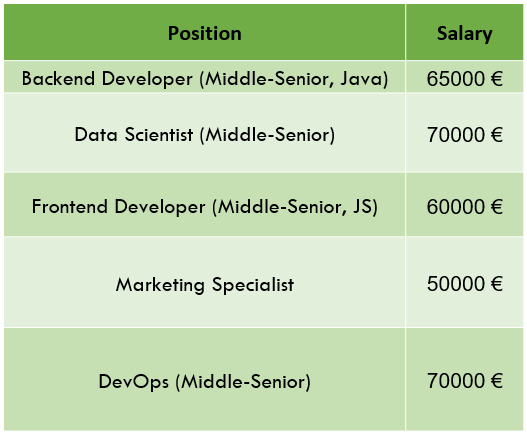
\includegraphics[width=0.5\textwidth]{figures/founder_salaries.png}
    \caption{Founders' foregone salaries}
    \label{fig:founder_salaries}
\end{figure}

In figure \ref{fig:founder_salaries} we can see salaries (brutto) for the position and experience level needed, according to Glassdoor \cite{glasdoor}.

\section{Cost structure}

The costs for this project can be classified into two camps: one-time payments and ongoing costs.

\p
There are following one-time payments:

\begin{itemize}
    \item Initial capital for GmbH - 25000€
    \item Initial marketing campaign - 10000€
    \item Initial tax advisor services - 2000€
    \item Initial lawyer expenses - 12000€
    \item Cloud costs for initial six months - 6000€
\end{itemize}

Tax advisor and lawyer expenses are estimated based on rates and workloads \cite{tax_advisor_rates}\cite{lawyer_rates}.

\p
There are following ongoing costs each month:

\begin{itemize}
    \item Cloud costs - 1000€
    \item Marketing campaign - 2000€
    \item License for YOLO - 416€ (5000€ per year) \cite{yolo_price}
    \item Expected lawyer costs - 500€
    \item Expected tax advisor costs - 50€
\end{itemize}

Cloud computing costs are estimated based on experience with projects of similar scale.

\p
Also, there are fees and taxes to include:

\begin{itemize}
    \item Marketplace fee - 15\% of subscription revenue \cite{google_play_fee}
    \item VAT - 19\%
    \item Corporate taxes - estimated at 30\% of profit
\end{itemize}

Corporate taxes consist of federal corporate tax (15\%) and trade tax, which varies based on residence. It's hard to estimate exactly, so it is a rough estimate.

\section{Expected performance}

There are following assumptions in the business plan presented below: the subscription rate is 20\%, churn rate for subscriptions is 50\% yearly, active users view 300 ads per month on average.

\p
As we can see from the table \ref{fig:budget} and graph \ref{fig:breakeven_no_salary}, we expect a net profit just in the 8th month. But given that the founders have foregone their salary, true breakeven point is in the end of the second year, as shown in graph \ref{fig:breakeven_salary}.

\begin{table}[]
    \resizebox{\textwidth}{!}{%
    \begin{tabular}{|l|l|l|l|l|l|l|l|l|l|l|l|l|}
        \hline
        Month & Customers & Subscriptions & \begin{tabular}[c]{@{}l@{}}Ad \\ revenue\end{tabular} & \begin{tabular}[c]{@{}l@{}}Subscription\\ revenue\end{tabular} & \begin{tabular}[c]{@{}l@{}}Summary\\ income\end{tabular} & \begin{tabular}[c]{@{}l@{}}Summary\\ expenses\end{tabular} & \begin{tabular}[c]{@{}l@{}}Summary\\ personal cost\end{tabular} & VAT        & Net Profit  & Corporate tax & Profit after tax & Personal profit \\ \hline
        0     & 0         & 0             & 0                                                     & 0                                                              & 0                                                        & 65000                                                      & 157500                                                          & -12350     & -65000      & 0             & -65000           & -222500         \\ \hline
        1     & 200       & 0             & 780                                                   & 0                                                              & 780                                                      & 68550                                                      & 183750                                                          & -12876.3   & -67770      & 0             & -67770           & -251520         \\ \hline
        2     & 400       & 40            & 1404                                                  & 510                                                            & 2694                                                     & 72100                                                      & 210000                                                          & -13187.14  & -69406      & 0             & -69406           & -279406         \\ \hline
        3     & 800       & 80            & 2808                                                  & 510                                                            & 6012                                                     & 75650                                                      & 236250                                                          & -13231.22  & -69638      & 0             & -69638           & -305888         \\ \hline
        4     & 1600      & 160           & 5616                                                  & 1020                                                           & 12648                                                    & 79200                                                      & 262500                                                          & -12644.88  & -66552      & 0             & -66552           & -329052         \\ \hline
        5     & 3200      & 320           & 11232                                                 & 2040                                                           & 25920                                                    & 82750                                                      & 288750                                                          & -10797.7   & -56830      & 0             & -56830           & -345580         \\ \hline
        6     & 6400      & 640           & 22464                                                 & 4080                                                           & 52464                                                    & 86300                                                      & 315000                                                          & -6428.84   & -33836      & 0             & -33836           & -348836         \\ \hline
        7     & 10000     & 1280          & 34008                                                 & 8160                                                           & 94632                                                    & 89850                                                      & 341250                                                          & 908.58     & 3873.42     & 1162.026      & 2711.394         & -338538.606     \\ \hline
        8     & 14000     & 2000          & 46800                                                 & 9180                                                           & 150612                                                   & 93400                                                      & 367500                                                          & 10870.28   & 46341.72    & 13902.516     & 32439.204        & -335060.796     \\ \hline
        9     & 17000     & 2800          & 55380                                                 & 10200                                                          & 216192                                                   & 96950                                                      & 393750                                                          & 22655.98   & 96586.02    & 28975.806     & 67610.214        & -326139.786     \\ \hline
        10    & 19500     & 3400          & 62790                                                 & 7650                                                           & 286632                                                   & 100500                                                     & 420000                                                          & 35365.08   & 150766.92   & 45230.076     & 105536.844       & -314463.156     \\ \hline
        11    & 21500     & 3900          & 68640                                                 & 6375                                                           & 361647                                                   & 104050                                                     & 446250                                                          & 48943.43   & 208653.57   & 62596.071     & 146057.499       & -300192.501     \\ \hline
        12    & 23000     & 4300          & 72930                                                 & 5100                                                           & 439677                                                   & 107600                                                     & 472500                                                          & 63094.63   & 268982.37   & 80694.711     & 188287.659       & -284212.341     \\ \hline
        13    & 24000     & 4600          & 75660                                                 & 3150                                                           & 518487                                                   & 116150                                                     & 498750                                                          & 76444.03   & 325892.97   & 97767.891     & 228125.079       & -270624.921     \\ \hline
        14    & 25000     & 4800          & 78780                                                 & 2550                                                           & 599817                                                   & 119700                                                     & 525000                                                          & 91222.23   & 388894.77   & 116668.431    & 272226.339       & -252773.661     \\ \hline
        15    & 26000     & 5000          & 81900                                                 & 2805                                                           & 684522                                                   & 123250                                                     & 551250                                                          & 106641.68  & 454630.32   & 136389.096    & 318241.224       & -233008.776     \\ \hline
        16    & 27000     & 5200          & 85020                                                 & 2805                                                           & 772347                                                   & 126800                                                     & 577500                                                          & 122653.93  & 522893.07   & 156867.921    & 366025.149       & -211474.851     \\ \hline
        17    & 28000     & 5400          & 88140                                                 & 3060                                                           & 863547                                                   & 130350                                                     & 603750                                                          & 139307.43  & 593889.57   & 178166.871    & 415722.699       & -188027.301     \\ \hline
        18    & 29000     & 5600          & 91260                                                 & 3570                                                           & 958377                                                   & 133900                                                     & 630000                                                          & 156650.63  & 667826.37   & 200347.911    & 467478.459       & -162521.541     \\ \hline
        19    & 30000     & 5800          & 94380                                                 & 4590                                                           & 1057347                                                  & 137450                                                     & 656250                                                          & 174780.43  & 745116.57   & 223534.971    & 521581.599       & -134668.401     \\ \hline
        20    & 31000     & 6000          & 97500                                                 & 6630                                                           & 1161477                                                  & 141000                                                     & 682500                                                          & 193890.63  & 826586.37   & 247975.911    & 578610.459       & -103889.541     \\ \hline
        21    & 32000     & 6200          & 100620                                                & 7140                                                           & 1269237                                                  & 144550                                                     & 708750                                                          & 213690.53  & 910996.47   & 273298.941    & 637697.529       & -71052.471      \\ \hline
        22    & 33000     & 6400          & 103740                                                & 7650                                                           & 1380627                                                  & 148100                                                     & 735000                                                          & 234180.13  & 998346.87   & 299504.061    & 698842.809       & -36157.191      \\ \hline
        23    & 34000     & 6600          & 106860                                                & 6375                                                           & 1493862                                                  & 151650                                                     & 761250                                                          & 255020.28  & 1087191.72  & 326157.516    & 761034.204       & -215.796        \\ \hline
        24    & 35000     & 6800          & 109980                                                & 5737.5                                                         & 1609579.5                                                & 155200                                                     & 787500                                                          & 276332.105 & 1178047.395 & 353414.2185   & 824633.1765      & 37133.1765      \\ \hline
        \end{tabular}}
    \caption{Planned business performance}
    \label{fig:budget}
\end{table}

\begin{figure}[H]
    \centering
    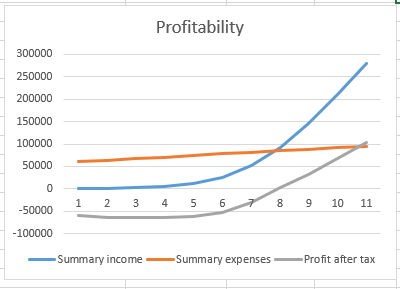
\includegraphics[width=0.5\textwidth]{figures/breakeven_no_salary.png}
    \caption{Breakeven point not including founder's personal cost}
    \label{fig:breakeven_no_salary}
\end{figure}

\begin{figure}[H]
    \centering
    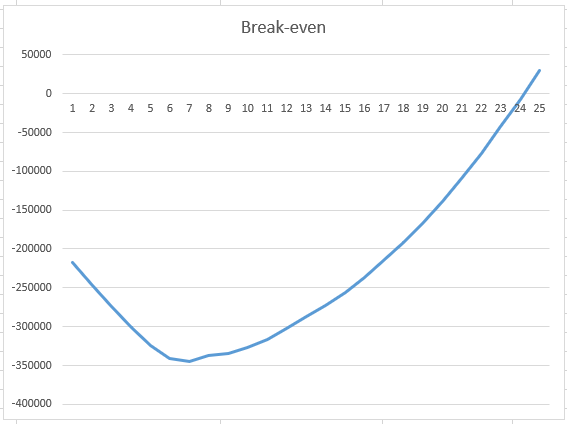
\includegraphics[width=0.5\textwidth]{figures/breakeven_salary.png}
    \caption{Breakeven point including founder's personal cost}
    \label{fig:breakeven_salary}
\end{figure}
	}

    % Marketing and sales: how will you sell it
	{
		\FloatBarrier
		\chapter{Marketing and sales: How to sell it?}
		\label{chp:marketing}
		by Polina Kozyr

\section{Marketing methods}

Our company needs advertising to make people aware of us. There are several ways to achieve recognition and sales for our company:

\begin{itemize}
    \item Digital Marketing

    Social Media Marketing: Leverage platforms like Instagram, Facebook, TikTok and Twitter to showcase the benefits of the app. We can use engaging content, such as videos and testimonials, to build brand awareness.
    
    Search Engine Optimization (SEO): Optimize the website and app store listings to rank higher in search engine results, making it easier for potential users to discover our app.
    \item Content Marketing

    Blog Posts and Articles: creation of informative blog posts or articles related to posture, health, and well-being. Sharing of practical tips and information that can attract target audience.
    
    Video Content: Development of instructional videos, product demonstrations, or educational content about the importance of maintaining good posture. Videos can be shared on social media, YouTube, and our website.
    \item Influencer Marketing
    
    We can enter into a partnership with influencers in the health and fitness space to promote our posture-controlling app. 
    \item Email Marketing
    
    Build an email list and send newsletters with valuable content, updates, and promotional offers. Email marketing is a direct way to engage with our audience and encourage app usage. But emails will only be used if people have given us permission to send them.
    \item Partnerships and Collaborations

    Formation of partnerships with health and wellness brands, fitness influencers, or ergonomic product manufacturers. Collaborations can enhance app's credibility and broaden its reach.
    \item App Store Optimization (ASO)
    
    Optimization of the app store listings with relevant keywords, compelling descriptions, and high-quality visuals. It is needed for increasing visibility on app stores and attracting downloads.
    \item Free Trials and Promotions

    Free trials to encourage users to try our app. Positive user experiences during trial periods can lead to increased subscriptions or purchases.
    \item Community Engagement

    Creation of online communities, forums, or social media groups where users can discuss posture-related topics, share experiences, and ask questions. Engaging with our community builds brand loyalty. We could make marathons like “21 day of straight posture”.
    \item Events and Sponsorships

    Attendance of wellness events, conferences, or trade shows. Participating in relevant events can provide exposure and networking opportunities.
    \item Leverage User Reviews

    Encouragement of satisfied users to leave positive reviews on app stores or provide testimonials for our marketing materials. 
\end{itemize}

\section{4Ps of marketing}

The 4Ps of marketing are a set of key elements that are considered essential in the development and execution of a marketing strategy. This analysis is presented in table 6.1.

\begin{table}[H]
    \centering
    \small
    \begin{tabular}{|c|c|}
        \hline
        \parbox{8cm}{\vspace{5pt}
        \textbf{PRODUCT}\\
        •	Intangible product - app\\
        •	Features: real-time posture monitoring, personalized feedback, posture reminder, user-friendly interface\\
        •	Our USP (unique selling point)\\
            “You don’t need to worry about your posture while focusing, we will evaluate and report on your posture for you!“\\
            "We will help you to develop a habit.“\\
            “Don’t interrupt your flow!”\\
        •	Needs: posture correction and constantly remembering about posture\\
        •	Marathons\\
        •	Healthy posture "club"\\
        •	Subscription\\
        •	Family subscription\\
        •	Business subscription models\\
        \vspace{5pt}} & \parbox{7cm}{\vspace{5pt}
        \textbf{PROMOTION}\\
        •	Create Instagram, Facebook and TikTok, WeChat, LinkedIn profiles with content that will be constantly updated\\
        •	Bloggers and influencers can promote the app for commission\\
        •	Paid advertising channels, such as Google Ads, Facebook Ads\\
        •	Family subscription that will have lower price per person than single-person subscription\\
        •	Price for subscription for six or twelve months at once will be cheaper\\
        •	Black Friday\\
        •	Cooperation with health insurances, physiotherapists   \\     
        \vspace{5pt}} \\
    \hline
    \parbox{8cm}{\vspace{5pt}
        \textbf{PRICE}\\
        •	Free trial period, e.g. 7 days\\
        •	Payment for subscription once in a month, six months, year\\
        •	Show the value: If you take care about posture now, you don't have to pay for medicine in the future\\
        •	Custom features for extra charge\\
        •	Multiple people subscription: family subscription\\  
        \vspace{5pt}} & \parbox{7cm}{\vspace{5pt}
        \textbf{PLACE}\\
        •	The app will be available on our website, App store and Google Play     
        \vspace{5pt}} \\
    \hline
    \end{tabular}
    \caption{4Ps of marketing}
\end{table}

\section{Analysis of customer groups}

Our customer base can be segmented based on various factors, including demographics, occupation, family status and income. Different groups of customers are presented in table 6.2.

\begin{table}[H]
    \centering
    \small 
    \begin{tabular}{|p{1.9cm}|p{2cm}|p{2cm}|p{2cm}|p{2.1cm}|p{2cm}|p{2cm}|}
        \hline
        \textbf{Criteria} & \textbf{Segment 1} & \textbf{Segment 2} & \textbf{Segment 3} & \textbf{Segment 4} & \textbf{Segment 5} & \textbf{Segment 6} \\
        \hline
        \textbf{Occupation} & Graduated, Employed & Graduated, Employed	& Students, Graduated or apprenticeship	& Apprenticeship, Students	& not employed, not students & E-Sports, Gamers \\
        \hline
        \textbf{Age} & 50-65 & 30-50 & 25-40 & 20-30 & 20-65 & 15-50 \\
        \hline
        \textbf{Family status} & Married, "Empty nest" & Married, with kids & Singles, married, with kids & Single & Married, Single, with kids & *\\
        \hline
        \textbf{Income} & 60.000-200.000 & 60.000-100.000 & 30.000-80.000 & 10.000-50.000 & * & 0-200.000\\
        \hline
    \end{tabular}
    \caption{Analysis of customer groups}
    \label{tab:example}
\end{table}

We use the “*” sign to denote irrelevant table cells.

\textbf{Group A}: Clients in this group (Segments 2, 3, and 6) are crucial for our company's success and revenue. Segment 3 comprises students, graduate students, and working individuals who spend significant time on computers, potentially experiencing back issues due to a sedentary lifestyle. Segment 2 shares similar characteristics but includes individuals which are employed and have families, possibly interested in a family subscription. Lastly, Segment 6 consists of professional competitive sports players who, while spending considerable time on computers, may benefit from posture tracking. All these segments have a common need to control their posture while working on the computer and have a regular income.

\textbf{Group B}: Customers in this group (Segments 1 and 4) are less likely to be initially interested in our product, but we aim to attract them. Segment 1 consists of working individuals, likely married, possibly less engaged in social media, and preferring traditional health care methods. Developing strategies to appeal to this segment is a future focus. Segment 4 includes students or trainees who are single, not currently concerned with posture correction. Future efforts may involve using bloggers and youth social networks to create engaging content emphasizing the importance of posture control for young individuals.

\textbf{Group C}: Clients in this group are unlikely to find our product relevant. This category consists of individuals who neither work nor study extensively on computers, indicating a limited need for our posture-controlling app.






	}

    % Competition: who else is in the game
	{
		\FloatBarrier
		\chapter{Competition: Who else is in the game?}
		\label{chp:competition}
		(by Nourhan Omar)

\p
Three possible competitors were found for Posefix, and while they are not based in Europe, 
the products are sold online and could easily be delivered to customers in Germany, whether in the form of software or a physical device.

\p
Below is the summary of the competitor's analysis:

\begin{table}[ht]
    \centering
    \begin{tabular}{|p{3cm}|p{3cm}|p{3cm}|p{3cm}|}
        \hline
        \textbf{Competitor} & \textbf{Zen} & \textbf{Posture AI} & \textbf{Upright} \\
        \hline
        Type & Software & Software & Physical Device \\
        \hline
        Device needed & Camera/Bluetooth headphones & Sensor/smart t-shirt & Sensor \\
        \hline
        Finances & Raised \$3.5M & 2 investors, still in beta phase & \$2.4M revenue/year, Acquired for \$31M \\
        \hline
        Target Customers & Consumers (B2C), Companies (B2B), Insurance Companies (B2B) & Consumers (B2C) & Consumers (B2C), Companies (B2B) \\
        \hline
        Pricing & Subscription-based model, \$9.99 - \$24.99 per year for consumers & One-time purchase: \$149 & One-time purchase: \$59.95-\$94.99 \\
        \hline
        Place & Online & Online & Online \\
        \hline
        Promotion & Online articles/social media & Online articles/website & Website/ articles/ social media \\
        \hline
        Skills & Cheap, easy access, bad UI & Expensive, had not fully launched, based in Seoul, Requires wearable (inconvenient) & Inconvenient wearable, good price, big market share, Android app store downloads \\
        \hline
    \end{tabular}
\end{table}    

\section{Zen}

\begin{figure}[H]
    \centering
    
\includegraphics[width=0.5\textwidth]{zen.png}
    \caption{Zen logo}
    \label{fig:zen}
\end{figure}

Zen is our main competitor as it has a very similar product to ours and is targeting similar customer groups as well. Zen is a software that detects your posture through the webcam if it's a desktop application or through the air pods if it's an iPhone application.  It was founded in October 2020 and is based in California in the United States \cite{zen_crunchbase}. It has raised $3.5$ million in 2021 from multiple investors including Y combinator\cite{posturehealth_ycombinator} and Valor Equity partners \cite{zen_techcrunch}. According to their LinkedIn\cite{posturehealth_linkedin} profile, they have tens of thousands of users. 

\p
Zen has a \$9.99 yearly subscription if it's the mobile version and \$24.99 if it's the desktop version. It targets consumers, companies as well as medical institutions such as hospitals and insurance companies. It advertises through paid online articles and paid partnerships with influencers on social media, but the ads are mainly focused on the mobile application.

\p
The good thing about Zen is that it's easily accessible on the phone as it can get downloaded from the Apple store and is cheap compared to other competitors. However, it takes a little digging to reach the desktop app, and the UI is non-intuitive making it hard to use. Additionally, it is mainly targeting customers in the US especially the companies and medical institutions.

\section{Posture AI}
\begin{figure}[H]
    \centering
    
\includegraphics[width=0.5\textwidth]{posture_ai.png}
    \caption{Posture AI logo}
    \label{fig:posture_ai}
\end{figure}

\begin{figure}[H]
    \centering
    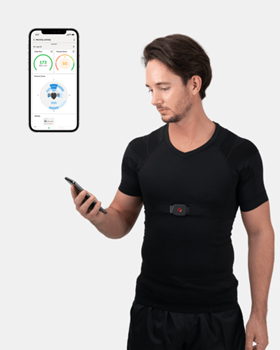
\includegraphics[width=0.5\textwidth]{wearable_ai.png}
    \caption{smart t-shirt}
    \label{fig:wearable_ai}
\end{figure}
Even though Posture AI launched 2 years ago and has 2 offices in Seoul \cite{postureai_linkedin} but the product is still in beta testing. It consists of a wearable t-shirt with a sensor that gets connected to a mobile application. The product is a one-time purchase at \$149 and could be ordered online through their website \cite{myposture}. The company mainly targets consumers and has 2 investors but they are not publicly known \cite{postureai_pitchbook}. The Android mobile app only has 50+ downloads. 

\p
The product promises to improve posture through the “functional” shirt with an ergonomic design and the sensor that tracks your posture and provides real-time feedback yet the device does not seem practical as it requires wearing the shirt all the time which is unrealistic. Additionally, due to the high price of the product, the consumer won't be able to buy multiples to switch between.

\section{Upright}

\begin{figure}[H]
    \centering
    
\includegraphics[width=0.5\textwidth]{upright_logo.png}
    \caption{Upright logo}
    \label{fig:upright_logo}
\end{figure}

Upright has been on the market since 2014 \cite{uprightpose} and has received hype on social media during COVID-19 when people started working from home and focusing on their posture.
Upright is a physical device that sticks to the back of the consumer and is connected to a mobile application that has over 50 thousand downloads in the Android app store.
It buzzes whenever the consumer slouches to instantly warn them to adjust their posture.
The product is promoted through their website and social media and earns \$2.4 million per year through selling their product \cite{upright_growjo} ranging from \$59.95 to \$79.95.
The price differs whether the consumer buys the device with 2 or 3 sensors and whether they buy the accessories set or the standalone device.
The company was acquired by Dario Health for \$31 million in 2021 \cite{dariohealth_acquisition}.

\begin{figure}[H]
    \centering
    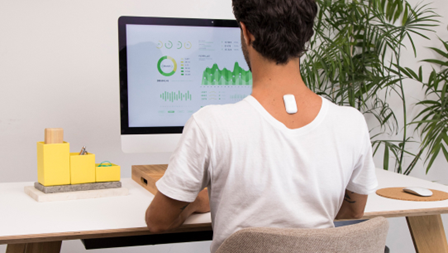
\includegraphics[width=0.5\textwidth]{upright_device.png}
    \caption{Upright Go 2 device}
    \label{fig:upright_device}
\end{figure}

The company is based in Israel but targets end consumers across the globe through its online website and selling through third-party such as Amazon. The cons of this product are that the consumer has to keep wearing the product and that it only targets one point in the body.

\section{Competitive Strategy}

Our competitive strategy is a differentiation focus strategy where we aim for our product to be a technological and user experience leader by providing the latest technologies to accurately detect the consumer's posture without the need for any external device or sensor other than the camera. 

\p
Additionally, we would focus on providing a better user experience by focusing on consumer privacy as well as providing leaderboard scores and competition badges to encourage consumers to keep using the application. We would also focus our strategy on the German market, especially German workplaces as none of our competitors are focusing on the German market yet.
	}

    % Implementation team: Who will implement the plan?
	{
		\FloatBarrier
		\chapter{Implementation team: Who will implement the plan?}
		\label{chp:implementation}
		(by Vipin Singh)

\p
This chapter presents an analysis of the team structure essential for executing the business model.
It outlines the various roles within the organization and their contributions towards achieving the business objectives.
The focus lies on understanding the division of responsibilities and the collaborative efforts necessary for the company's growth and success.
This examination is intended to provide a clear view of the organizational framework and its significance in the operational realization of the business strategy.

\section{Team composition in the startup phase}
\label{sec:team_comp_startup}
Since the business idea will start in a small scale, the human resources need to be used as efficiently as possible.
With only five founder members, this requires that each members role is not just defined by their job title.
Instead each member will have to be able to adapt and contribute across various facets of the business.
Still the business should also be able to scale up and expand its operations as it grows.

\p
With this said lets analyze the team composition, that is focused to rapidly develop and launch the product.

%TODO: Maybe create the table inline?
\begin{figure}[H]
    \centering
    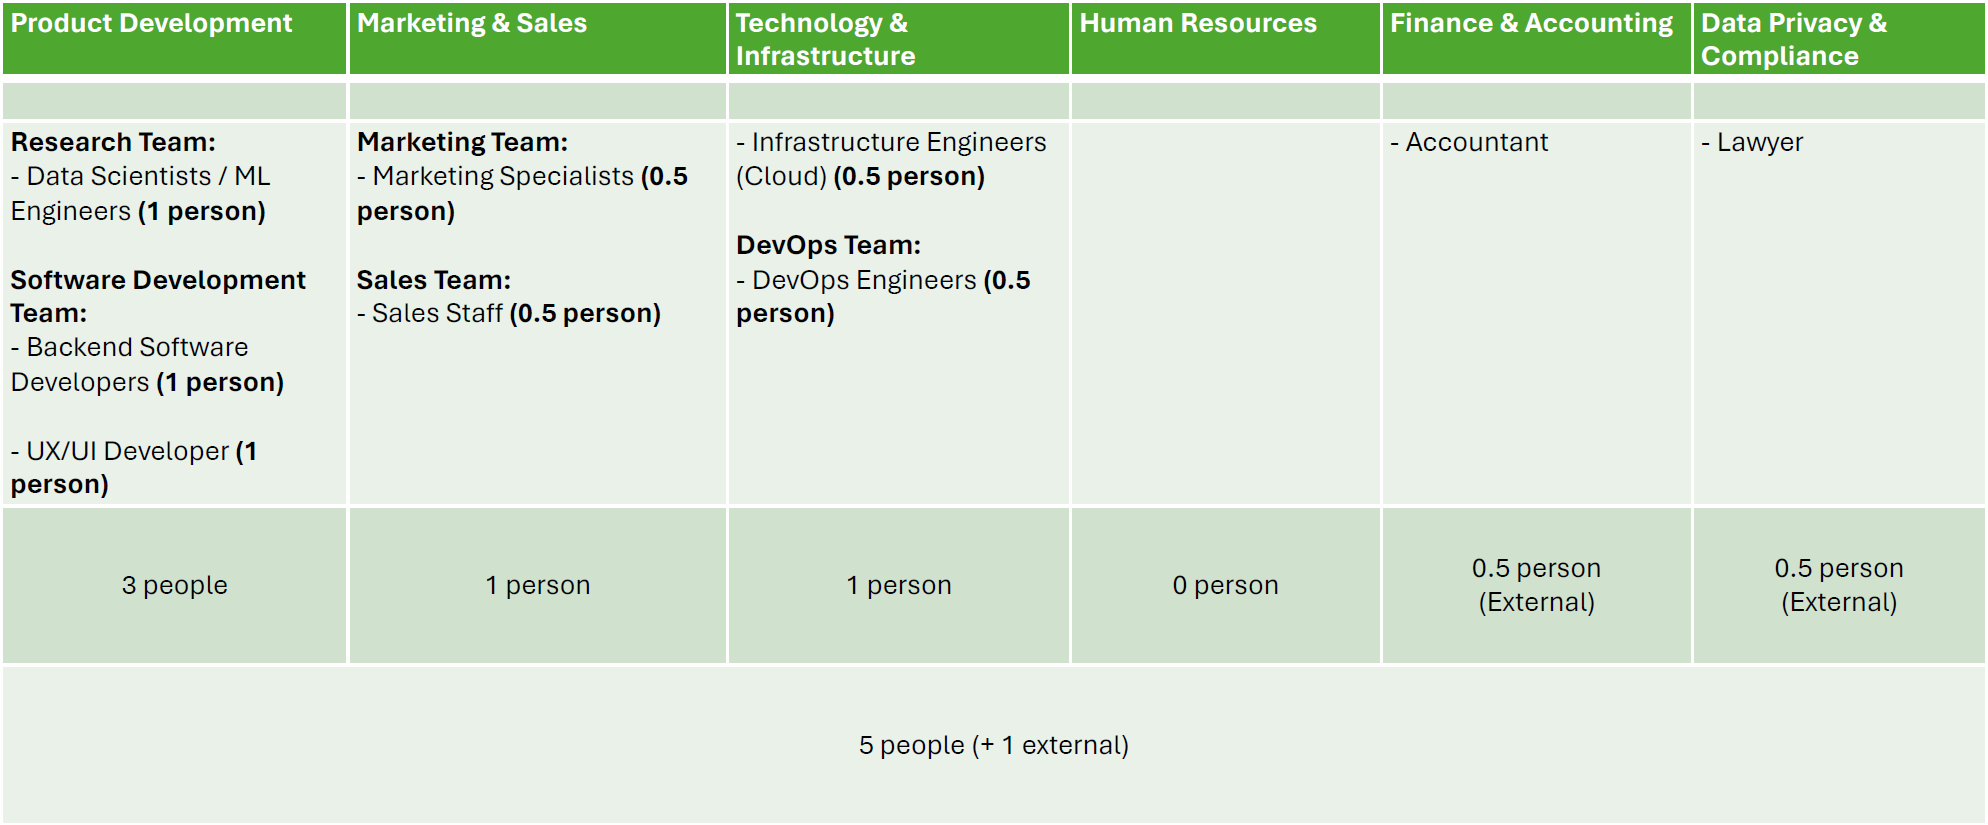
\includegraphics[width=\textwidth]{figures/team_comp_startup.png}
    \caption{Departments with team composition for a startup}
    \label{fig:team_comp_startup}
\end{figure}

In figure \ref{fig:team_comp_startup} we can see the team composition for a startup.
We decided to split the implementation of the team composition into six departments.
This department structure helps us to better understand the responsibilities we must fulfill for the business idea to succeed.
As we assign three out of the five founders to the product development department, it becomes clear that this is the core of our business for launching the product as fast as possible.

\p
Before we start with explaining the decisions for the team composition in figure \ref{fig:team_comp_startup}, we want to explain the responsibilities of each department and each role within the departments.
We will continue with the explanation of the decisions in subsection \ref{sub:decision_on_team_comp_startup}.

\subsection{Department: Product Development}
The \textbf{Product Development} department serves as the core of innovation in our company.
It is responsible for designing the product by converting research insights into practical features.
It also ensures that the product is developed such that it meets the markets demand and holds the technical superiority over its competitors.
It is split into two teams, the Research team and the Software Development team.

\subsubsection*{Research Team}
The research team guides the development of new product features by providing insights into the latest research in the field of ergonomics and posture detection.
Therefore they are mainly responsible for the machine learning pipeline.
\begin{itemize}
    \item \textbf{Data Scientists / ML Engineers:}
            \begin{itemize}
                \item Keep track of foundation models for the task
                \item Analyze data to improve prediction accuracy for the posture keypoints
                \item Finetune the foundation models for our specific tasks with collected data
                \item Collaborate with software developers to integrate the machine learning pipeline into the product
            \end{itemize}
\end{itemize}

\subsubsection*{Software Development Team}
The software development team directly implements the product features into the codebase.
They also ensure that the product is scalable and maintainable, while having the user experience in mind.
Another important task that is not mentioned directly in the following is the testing of the products features and the documentation of the codebase.
\begin{itemize}
    \item \textbf{Backend Software Developers:}
            \begin{itemize}
                \item Write and maintain the codebase
                \item Implement new features
                \item Ensure scalability
            \end{itemize}
    \item \textbf{UX/UI Developer:}
            \begin{itemize}
                \item Design the user interface
                \item Design prototypes for new features
                \item Implement the designs for the user interface into the codebase
            \end{itemize}
\end{itemize}

\subsection{Department: Marketing \& Sales}
The \textbf{Marketing \& Sales} department functions as a crucial link between the product and the potential customers.
Its primary responsibilities are the development of marketing strategies that communicate the value proposition of the product to the target audience.
Furthermore they drive the sales initiatives to convert prospects into customers.
This is critical to generate revenue for the company.
The alignment of marketing and sales efforts ensure the customer acquisition and retention, which is vital for growth and success.
For further structure this department is split into two teams, the Marketing team and the Sales team.

\subsubsection*{Marketing Team}
The marketing team is responsible for adjusting and exeecuting the marketing strategies and also monitoring the marketing trends.
\begin{itemize}
    \item \textbf{Marketing Specialists:}
            \begin{itemize}
                \item Execute marketing campaigns
                \item Analyze campaign performance
                \item Manage content creation
                \item Design marketing media (e.g. flyers, posters, etc.)
                \item Ensure brand consistency
            \end{itemize}
\end{itemize}

\subsubsection*{Sales Team}
The sales team is responsible for the customer relationships and to identify potential customer segments.
Additionally they are togeether with the marketing team responsible to reach out to high potential customer segments.
\begin{itemize}
    \item \textbf{Sales Staff:}
            \begin{itemize}
                \item Reach out to potential clients
                \item Conduct sales pitches
                \item Negotiate contracts with B2B customers and close deals
            \end{itemize}
\end{itemize}

\subsection{Department: Technology \& Infrastructure}
The \textbf{Technology \& Infrastructure} serves as the foundational support for the company's internal operations.
This department ensures that the product is built on a reliable and advanced technological base.
Additionally they guarantee for uninterrupted service delivery and scalability internally but also for the customers.
The dual focus is crucial for the future growth of the company, allowing it to adapt to an evolving technological landscape.
They also setup systems for the company's employeees to work efficiently in projects.
\begin{itemize}
    \item \textbf{IT Support Staff:}
            \begin{itemize}
                \item Technical support to employees
                \item Perform maintenance and update on company hardware and software infrastructure
            \end{itemize}
    \item \textbf{DevOps Engineers:}
            \begin{itemize}
                \item Develop and maintain CI/CD (Continuous Integration/Continuous Development) pipelines
                \item Collaborate with software developers on code releases and deployments
                \item Implement automation tools to reduce manual processes
                \item Implement physical and network infrastructure to operate services
                \item Optimize the compute infrastructure and data storage
                \item Devlop and implement network security policies and procedures against unauthorized access
            \end{itemize}
\end{itemize}

\subsection{Department: Human Resources}
The \textbf{Human Resources} department plays a vital role in shaping the organization's talent and culture.
This department focuses primarily on recruiting skilled individuals who can contribute to the company's growth.
Additionally, the department is responsible for implementing training programs to enhance the employees' skills and knowledge.
They are also taking care of the administrative tasks, such as the employees' time registration and their holidays.

\subsection{Department: Finance \& Accounting}
The \textbf{Finance \& Accounting} department is there to maintain the financial integrity of the company.
Its primary responsibilities involve the comprehensive management of the company's finances.
This includes tasks such as budgeting (efficient allocation of resources), financial reporting (transparency of fiscal health), and accounting (accuracy and reliability of financial documentation).
Additionally, the department is tasked with overseeing the financial compliance, such as adherence to the tax regulations.
Furthermore, the department plays a role in optimizing financial planning and execution.
This is an essential prerequisite for the long-term growth and success of the company.

\begin{itemize}
    \item \textbf{Accountants:}
    \begin{itemize}
        \item Manage transactions and financial records
        \item Create invoices for the B2B customers according to the negotiations of the sales team
        \item Prepare tax returns and payments
        \item Maintain compliance with tax regulations
    \end{itemize}
\end{itemize}

\subsection{Department: Data Privacy \& Compliance}
The \textbf{Data Privacy \& Compliance} department is essential for ensuring the company's adherence to data protection laws and industry regulations.
Their primary tasks include maintaining compliance across the company's operations and preparing for the implementation of ISO certification guidelines.
This department plays a key role in upholding data ethics and legal conformity, crucial for the company's integrity and trustworthiness.

\begin{itemize}
    \item \textbf{Lawyer:}
            \begin{itemize}
                \item Ensure compliance with relevant laws and regulations
                \item Review business contracts and provide support in disputes
            \end{itemize}
\end{itemize}

\subsection{Decisions on the team composition for the startup phase}
\label{sub:decision_on_team_comp_startup}

In this subsection we want to explain the decisions we made for the team composition in figure \ref{fig:team_comp_startup}.
As already mentioned, since the main goal of the startup phase is to launch the product as fast as possible, we decided to assign three out of the five founders to the Product Development department.
The roles that are assigned in the product development department are the following:
\begin{itemize}
    \item Data Scientist / ML Engineer \textbf{(1 person)}
    \item Backend Software Developer \textbf{(1 person)}
    \item UX/UI Developer \textbf{(1 person)}
\end{itemize}
With these we have covered the most important roles in order to develop the first prototypes and develop these further to a product that can be launched.

These three members will need to work closely together and engage in a broader scope of tasks beyond just their dedicated roles to effectively develop the product in a small team.

\p
The remaining two founders are assigned to the Marketing \& Sales department and the Technology \& Infrastructure department.
Lets first look at the Marketing \& Sales department:
\begin{itemize}
    \item Marketing Specialist \textbf{(0.5 person)}
    \item Sales Staff \textbf{(0.5 person)}
\end{itemize}
Be aware that we assign only one person to the Marketing \& Sales department because we assume that one person working as both Marketing Specialist and Sales Staff is enough for the startup phase.
We also considered that the person working in this department will closely work together members of the Product Development department, especially with the UX/UI Developer.
They can together create marketing strategies to promote the product with the first prototypes and also create marketing media, such as flyers and posters.

\p
As mentioned the last founder is assigned to the Technology \& Infrastructure department:
\begin{itemize}
    \item Infrastructure Engineer \textbf{(0.5 person)}
    \item DevOps Engineer \textbf{(0.5 person)}
\end{itemize}
Similar to the Marketing \& Sales department we assign only one person to the Technology \& Infrastructure department because we assume that one person working as both Infrastructure Engineer and DevOps Engineer is enough for the startup phase.
The member working in this department will work closely together with the Backend Software Developer to setup the infrastructure for the product.

\p
The remaining departments, Human Resources, Finance \& Accounting and Data Privacy \& Compliance, are not assigned to any of the founders.
For the case of the Human Resources department we assume that the founders will take care of the administrative tasks, such as time registration and their holidays.
In that case there is no need for any employee in the Human Resources department.

\p
For the remaining two departments we seek to outsource the tasks to external companies.
For the Finance \& Accounting department we will outsource the tasks to an external accounting company, that will take care of the financial integrity of the company.
For the Data Privacy \& Compliance department we will outsource the tasks to an external lawyer, that will help us to ensure the company's adherence to data protection laws and industry regulations.

\p
With this we have covered all the departments and the roles within the departments for the startup phase.
We should be able to launch the product with this team composition of the five founder members.
After the product is launched we can start to scale up the company and hire more employees.
This leads to the next section \ref{sec:team_comp_highscaled}, where we will analyze the team composition after the company has scaled up.

\section{Team composition after higher scaling}
\label{sec:team_comp_highscaled}

In figure \ref{fig:team_comp_highscaled} we see how the team composition could look like after the company scaled up to a medium sized company.
As we can see, we have many more diverse roles in every department, allowing every single employee to work on their dedicated role.
In total in this team composition we propose 37 employees.

\begin{figure}[H]
    \centering
    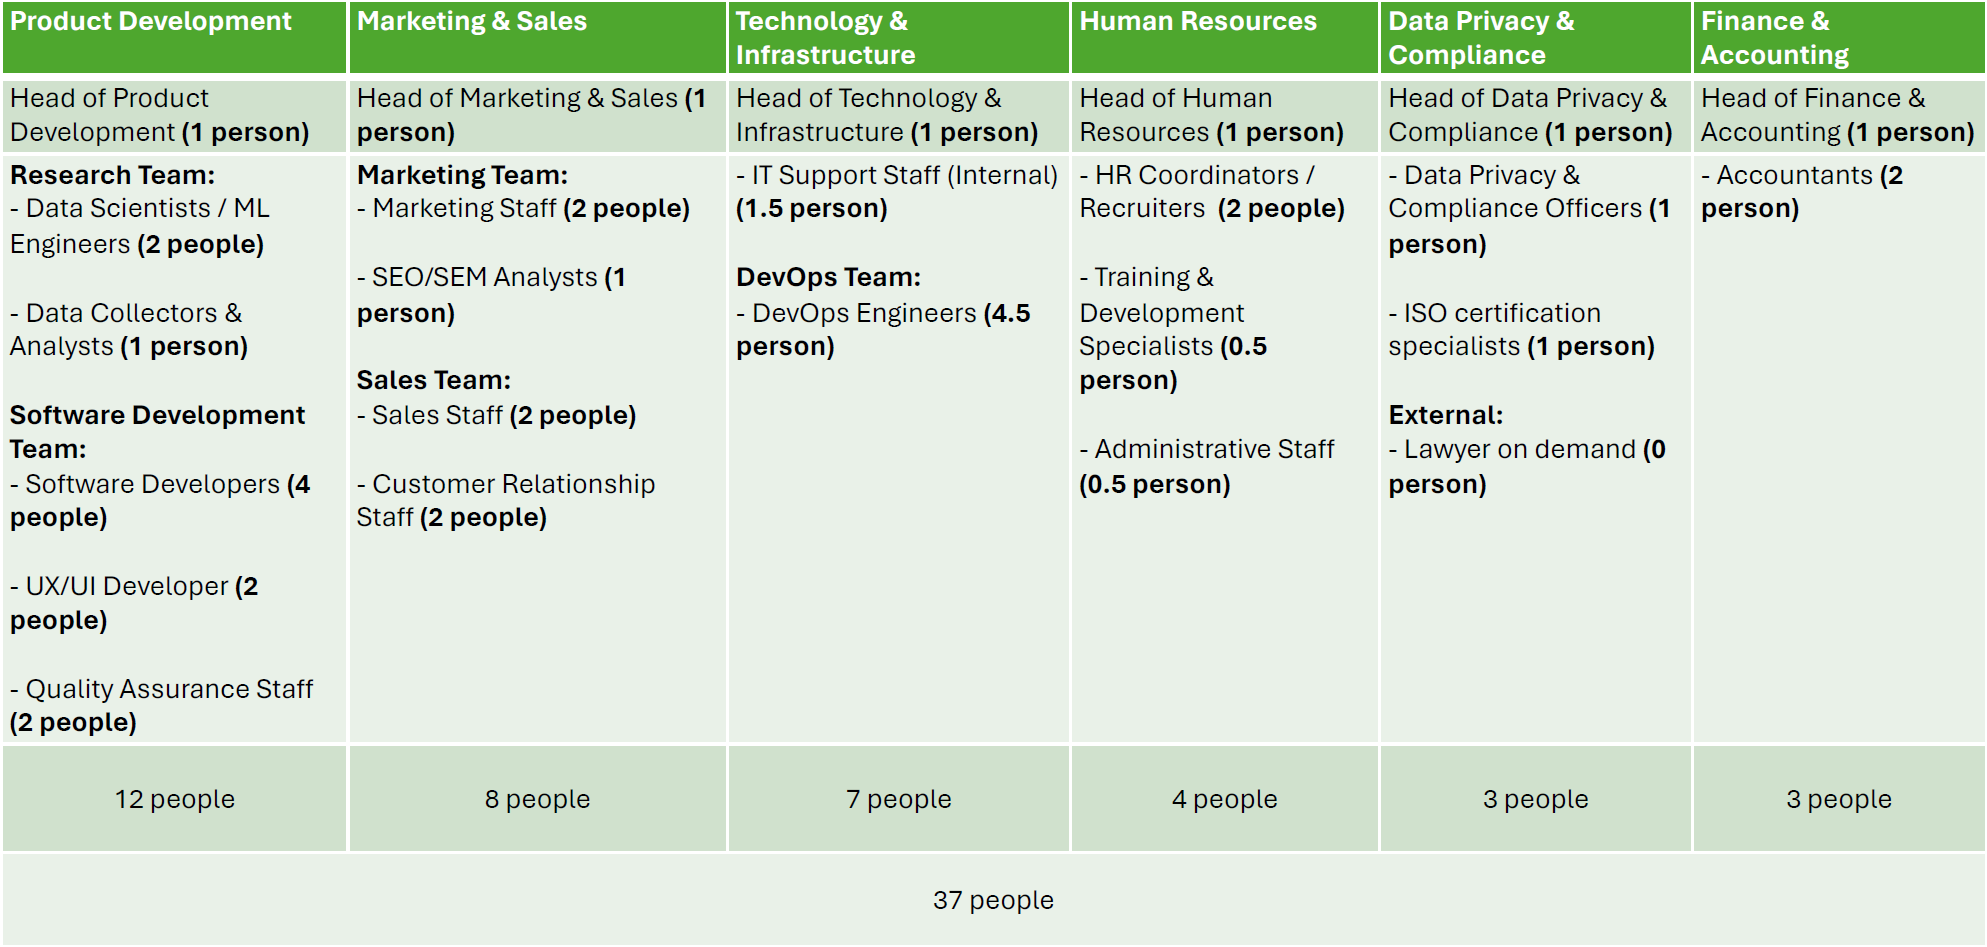
\includegraphics[width=\textwidth]{figures/team_comp_highscaled.png}
    \caption{Departments with team composition after the company has scaled up}
    \label{fig:team_comp_highscaled}
\end{figure}

Just as in section \ref{sec:team_comp_startup} we will explain each of the roles in the departments, before explaining the decisions.
Since the tasks of the roles that were already explained in section \ref{sec:team_comp_startup} are the almost the same, we will just explain the newly added roles.
The same applies for the description of the departments.

\subsection{Department: Product Development}
\begin{itemize}
    \item \textbf{Head of Product Development}
            \begin{itemize}
                \item Manage the product roadmap to achieve business goals
                \item Guide new product features development
                \item Collaborate with other department heads
            \end{itemize}    
\end{itemize}

\subsubsection*{Research Team}
\begin{itemize}
    \item \textbf{Data Collectors \& Analysts:}
            \begin{itemize}
                \item Collect data on user postures
                \item Process data for downstream tasks
                \item Collaborate closely with the Data Scientists / ML Engineers on the data analyses
            \end{itemize}
\end{itemize}

\subsubsection*{Software Development Team}
\begin{itemize}
    \item \textbf{Quality Assurance Staff:}
            \begin{itemize}
                \item Extensively test the app and new features
                \item Automate testing processes
                \item Documentation of issues
                \item Collaborate with the customer relationship staff for customer feedback
            \end{itemize}    
\end{itemize}

\subsection{Department: Marketing \& Sales}
\begin{itemize}
    \item \textbf{Head of Marketing \& Sales}
            \begin{itemize}
                \item Monitor marketing trends
                \item Adjust marketing strategies
                \item Direct B2B related marketing
                \item Collaborate with other department heads
            \end{itemize}    
\end{itemize}

\subsubsection*{Marketing Team}
\begin{itemize}
    \item \textbf{SEO/SEM Analysts:}
            \begin{itemize}
                \item Coordinate SEO (search engine optimization) and SEM (search engine marketing)
                \item Analyze digital performance of our marketing channels
            \end{itemize}
\end{itemize}

\subsubsection*{Sales Team}
\begin{itemize}
    \item \textbf{Customer Relationship Staff:}
            \begin{itemize}
                \item Build/Maintain relationships with customers (specifically B2B customers)
                \item Retrieve feedback from the customers to develop issues for the quality assurance
                \item Identify upselling opportunities
            \end{itemize}
\end{itemize}

\subsection{Department: Technology \& Infrastructure}
\begin{itemize}
    \item \textbf{Head of Technology \& Infrastructure:}
            \begin{itemize}
                \item Manage technical direction of the company
                \item Manage the team's project planning
                \item Collaborate with other department heads
            \end{itemize}    
\end{itemize}

\subsection{Department: Human Resources}
\begin{itemize}
    \item \textbf{Head of Human Resources:}
            \begin{itemize}
                \item Develop and discuss HR strategies to succeed with the business idea
                \item Collaborate with other department heads
            \end{itemize}
    \item \textbf{HR Coordinators / Recruiters:}
            \begin{itemize}
                \item Assist with recruitment
                \item Identify staffing needs
                \item Create job descriptions
            \end{itemize}
    \item \textbf{Training \& Development Specialists:}
            \begin{itemize}
                \item Create training strategies to enhance employees’ skills
            \end{itemize}    
    \item \textbf{Administrative Staff:}
            \begin{itemize}
                \item Manage employees' time registration and holidays
            \end{itemize}    
\end{itemize}

\subsection{Department: Data Privacy \& Compliance}
\begin{itemize}
    \item \textbf{Head of Data Privacy \& Compliance:}
            \begin{itemize}
                \item Lead the team
                \item Collaborate with other department heads
            \end{itemize}    
    \item \textbf{Data Privacy \& Compliance Officers:}
            \begin{itemize}
                \item Monitor and improve company’s data protection strategies
                \item Ensure GDPR compliance
                \item Oversee company’s structure to prevent violations of legal guidelines
                \item Ensure internal guidelines are being followed
                \item Collaborate with HR coordinators
            \end{itemize}
    \item \textbf{ISO Certification Specialists:}
            \begin{itemize}
                \item Guide the company through the ISO certification process
                \item Maintain compliance with ISO standards
            \end{itemize}
\end{itemize}

\subsection{Department: Finance \& Accounting}
\begin{itemize}
    \item \textbf{Head of Finance \& Accounting:}
            \begin{itemize}
                \item Financial planning and strategy of the company
                \item Analyze financial data
                \item Budget forecasting and financial statements
                \item Develop financial models
                \item Collaborate closely with accountants
                \item Collaborate with other department heads
            \end{itemize}
\end{itemize}

\subsection{Decisions on the team composition after higher scaling}
\label{sub:decision_on_team_comp_highscaled}

In this new team composition with many more employees we added the roles of the heads of the departments, as a management position.
We see the necessity of these roles, because the company has grown and we need to have a clear structure, so that the departments can work together efficiently.
The heads of the departments are responsible for collaboration with the other department heads and serve as a link between the departments.

\p
Lets start analyzing the team composition first with the Product Development department.
In this department the Software Development team had a large increase in employees.
This should help to scale and improve the product faster.
We also added a Quality Assurance Staff, that is responsible for testing the product and new features, this helps the software developers to focus on developing.
This department still is the biggest department in the company, to ensure that we remain innovative to stay ahead of the competition.

\p
In the Marketing \& Sales department we now have more specified roles in both the Marketing team and the Sales team.
The team sizes are still small, because we want to keep the company agile and flexible.

\p
With a larger company we also have much more need of a better infrastructure.
Therefore we added a lot of DevOps Engineers that also take care of the internal IT support.
This helps to optimize the internal processes and secure the company's data.

\p
With more employees a Human Resources department also becomes important to manage the employees and the staffing needs.
For enhancing the employees' skills we added a Training \& Development Specialist, that also takes care of the administrative tasks.
So we decided to add four employees to the Human Resources department.

\p
The Data Privacy \& Compliance department now has internal employees, that take care of the data protection and the ISO certification.
The ISO certification is an important step for the company to ensure the quality of the product and the company's processes.
From previous experience we know that the ISO certification process is very time consuming, therefore we added one employees only dedicated to the ISO certification.
Since we do not have employees with a lawyer background, we decided to outsource important legal tasks to an external lawyer, that we will consult on demand.

\p
For managing the company's finances we also added internal employees to the Finance \& Accounting department.
With the accountants taking care of financial records and tax returns, the Head of Finance \& Accounting can focus on analyzing the financial data and develop financial models.
This helps to optimize the company's financial planning and strategy.

\p
With this we have covered all the departments and the roles within the departments for the team composition after the company has scaled up.
Our most important thoughts for this team composition were to keep the company agile and flexible, so that we can adapt to the market and stay ahead of the competition.
To conclude this chapter, we can state that a company with more employees must also have a clear structure so that the departments can work together efficiently.
	}

    % Status or timeline: Where are we now, what next?
	{
		\FloatBarrier
		\chapter{Status or timeline: Where are we now, what next?}
		\label{chp:timeline}
		(by Vipin Singh)

\p
In this chapter we will discuss the timeline of the project, for which we show a GANTT chart in figure \ref{fig:timeline_gantt} showing the roadmap for implementing the business idea.

\begin{figure}[H]
    \centering
    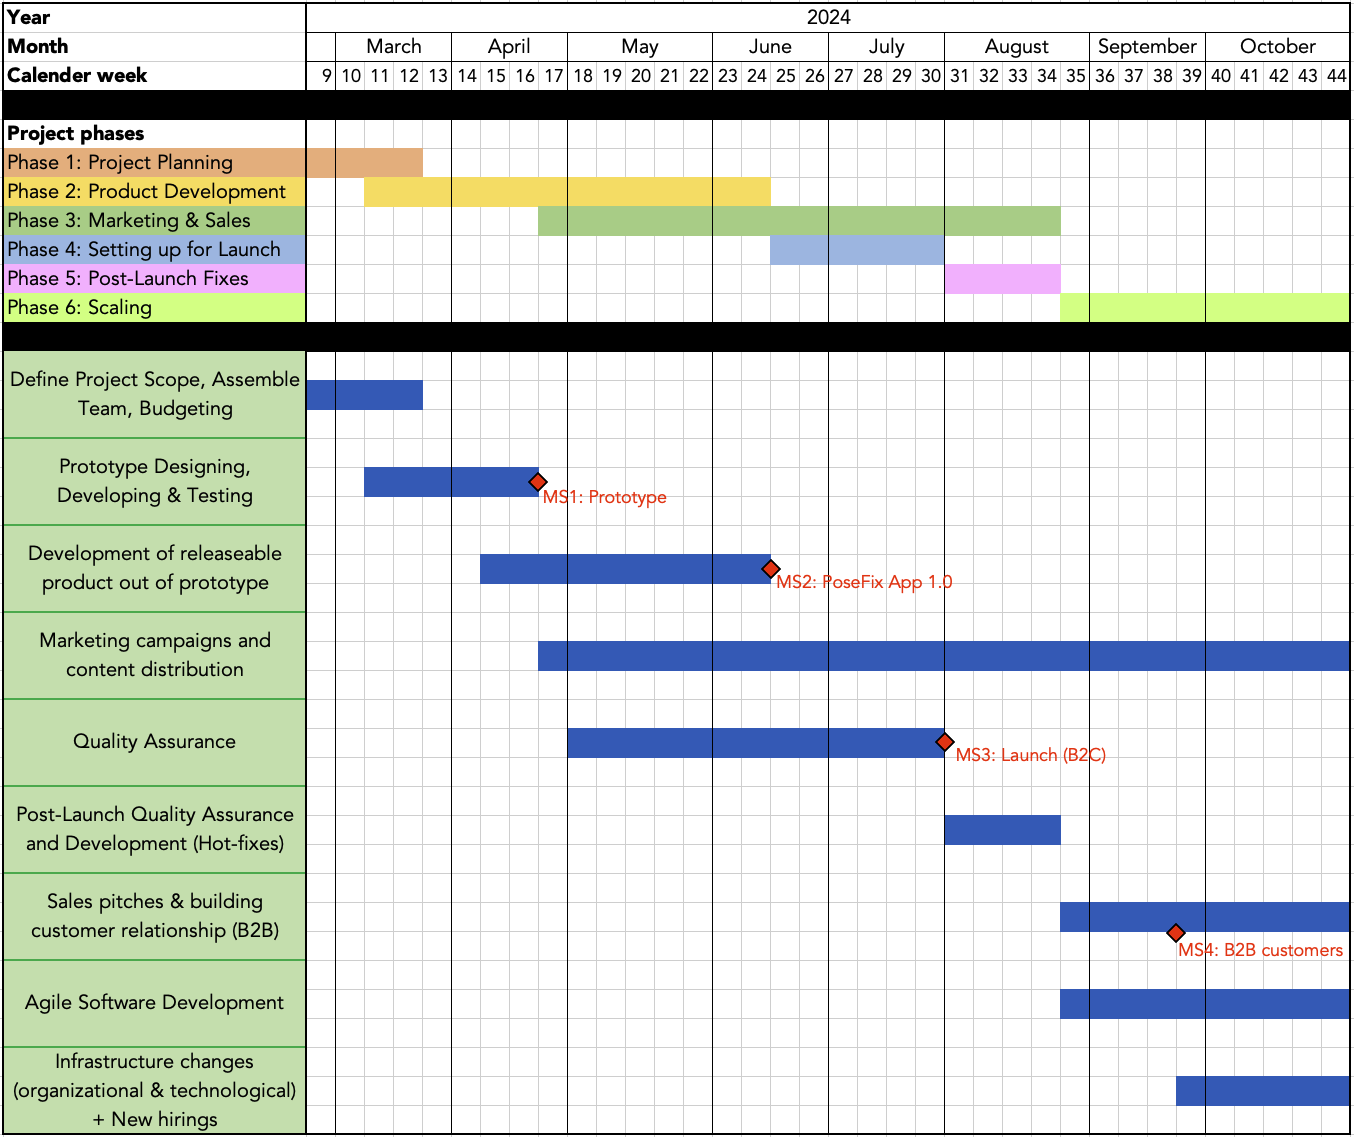
\includegraphics[width=\textwidth]{figures/GANTT_timeline.png}
    \caption{Timeline of the project as a GANTT chart}
    \label{fig:timeline_gantt}
\end{figure}

To have a clear structure of the project, we mapped the different task into six phases.
The first phase is the \textbf{Project Planning} phase.
This phase will be used to set up the project teams, define the scope of the project and already start with budgeting.
In total we planned to spend 4 weeks on this phase.
After 2 weeks though we might be already able to start with the next phase.

\p
The second phase is the \textbf{Product Development}.
This phase will start with designing the prototype.
The initial designs of the prototype can also therefore already be discussed in the project planning phase.
After the design has been agreed on, the Product Development team can start developing and testing the prototype.
In total we assume that this task will take 6 weeks.
The prototype is also our first milestone in this project.
As soon as the prototype is ready, the next phase can start, while the Product Development phase continues.
A few weeks before the actual prototype is finalized the Product Development team can already start with the task of creating a releasable product out of the prototype.
From this point we expect the development of the first version of our product to take 10 weeks.
This then results in the second milestone of the project.
We call that milestone \textbf{PoseFix App 1.0}.
In total we expect the initial Product Development phase to take 14 weeks.

\p
The third phase \textbf{Marketing \& Sales} will start after 6 weeks of project start.
In this phase we can start developing marketing campaigns and start distributing content of our prototype on several channels, such as social media.
Since Marketing campaigns and content distribution should be an continuous process throughout the business, we consider this task to go on for the whole duration of the project.
Still we want to note that the strategies for Marketing \& Sales keep changing with further progress of the project, for example when the product is launched.

\p
Soon after the prototype is ready and the development of the launch version of the product has started, the quality assurance tasks should begin.
This should ensure that the product quality is high already when the product is launched.
In the GANTT chart we plan that the quality assurance task starts after 3 weeks of product development.
This is also the main task of the fourth phase \textbf{Setting up for Launch}.
This phase will start as soon as the first version of the product is ready.
It consists not only of quality assurance, but also Marketing \& Sales tasks.
This phase will end with our third milestone, the \textbf{Launch} of our product in the B2C market.
We assume that setting up for launch and adjusting the product will take 6 weeks after the first version of the product is ready.
In the timeline we are at this point 21 weeks or roughly 5 months into the project.

\p
As soon as the product is launched, one of the most stressful phases of the project will start.
The fifth phase is called \textbf{Post-Launch Fixes}.
With more and more users using our product, we will start getting actual feedback from our customers.
To maintain the high quality and to keep our customers happy, we will have to fix bugs and improve the product as fast as possible.
This is covered in the task "Post-Launch Quality Assurance and Development (Hot-fixes)".
We assume that this task will take 4 weeks, until the product is at a stable state, that a large amount of customers can enjoy.

\p
After the product is stable and becomes reliable we can start with the sixth and last phase of the project: \textbf{Scaling}.
In this phase we want to scale our business and grow our customer base.
This phase will be continuing even after the time span of the GANTT chart.
The tasks for this phase are further improving our product in agile fashion, developing new features and scaling our marketing campaigns.
The main task of this phase is also to get into the B2B market with our product.
The entry into the B2B market is therefore our fourth and last defined milestone in this timeline.
As soon as we start selling the product to companies and the normal customers we can consider our project as a success.
With the success of the project we can start with organizational and technological infrastructure changes and new hirings.
At this point we want to emphasize our goal to scale with the company to a medium sized company as already discussed in section \ref{sec:team_comp_highscaled}.

\p
With this we have concluded a timeline for our project, that focused on deploying our PoseFix App to the B2C and B2B market and scaling our business.
	}

    % Executive summary: Concise overview of the opportunity
	{
		\FloatBarrier
		\chapter{Executive summary: Concise overview of the opportunity}
		\label{chp:summary}
		(by Pavlo Kravets)

\p
The project that was detailed in this report is a promising development. It offers much better scalabilty than a typical computer vision startup due to solution being mostly client-side. It taps into underdeveloped market with few competitors. It provides a solution to a problem that will only grow bigger as society ages and becomes more sedentiary.

\p
Initial investment and projected maximum loss are low as startups go - only 60000€ and 65000€. This is not a blitzscaler that wil continue burning through the money for decades to come. In the world, where interest rates are no longer indestinguishible from zero, more steady and methodic approach is much more sensible.

\p
It would also be important to note, that the estimations provided in the report are conservative in a number of ways. For example, it does not take into account various incubator programs, such as one provided by the BHT, while it could save a lot of expenses, such as providing infrastructure or legal guidance, as well as partially compensating lost salaries. 

\p
Overall, this project has a potential. A potential to be Germany's new hidden gem company - not a flashy name that would provoke a hundred imitators, but simply a team of professionals that are the best at what they do. And Germany would be wise to support it.
	}

    % References
	{
		\FloatBarrier
		\newpage
		\phantomsection
		\addcontentsline{toc}{chapter}{References}
		\printbibliography[title = References]
	}

\end{document}
